%%
%% hibari_tda_report.tex — 한국어 보고서 형식
%% xelatex로 컴파일:
%%   xelatex hibari_tda_report.tex
%%   xelatex hibari_tda_report.tex   (cross-reference 해소용 2회)
%%

\documentclass[11pt,a4paper]{article}

% ── Packages ─────────────────────────────────────────────────────────────
\usepackage[margin=2.5cm]{geometry}
\usepackage{setspace}
\usepackage{amsmath, amssymb, amsthm}
\usepackage{graphicx}
\usepackage{booktabs}
\usepackage{multirow}
\usepackage{url}
\usepackage[hidelinks]{hyperref}
\usepackage{xcolor}
\usepackage{enumitem}
\usepackage{float}
\usepackage{caption}
\usepackage{fancyhdr}
\usepackage{titlesec}

% ── Korean font support (xelatex) ───────────────────────────────────────
\usepackage{fontspec}
\usepackage{xeCJK}
\setCJKmainfont{Malgun Gothic}
\setCJKsansfont{Malgun Gothic}
\setCJKmonofont{Malgun Gothic}

% ── Line spacing ─────────────────────────────────────────────────────────
\onehalfspacing

% ── Header/Footer ────────────────────────────────────────────────────────
\pagestyle{fancy}
\fancyhf{}
\fancyhead[L]{\small\leftmark}
\fancyhead[R]{\small\thepage}
\renewcommand{\headrulewidth}{0.4pt}

% ── Section formatting ───────────────────────────────────────────────────
\titleformat{\section}{\Large\bfseries}{\thesection.}{0.5em}{}
\titleformat{\subsection}{\large\bfseries}{\thesubsection}{0.5em}{}
\titleformat{\subsubsection}{\normalsize\bfseries}{\thesubsubsection}{0.5em}{}

% ── Theorem environments ─────────────────────────────────────────────────
\newtheorem{definition}{정의}[section]
\newtheorem{theorem}{정리}[section]
\newtheorem{remark}{비고}[section]

% ── Paths ────────────────────────────────────────────────────────────────
\graphicspath{{../figures/}}

% ── Caption style ────────────────────────────────────────────────────────
\captionsetup{font=small, labelfont=bf, skip=8pt}

% ── Title ────────────────────────────────────────────────────────────────
\title{%
\vspace{-1cm}
{\LARGE\bfseries
사카모토 류이치의 \emph{hibari}에 대한 위상적 데이터 분석}\\[0.4cm]
{\Large Persistent Homology 기반 구조 보존 음악 생성 파이프라인}
}

\author{%
\textbf{김민주}\\[0.2cm]
초학제 독립연구단\\
고등과학원 (KIAS)\\
서울, 대한민국
}

\date{2026}

% ═════════════════════════════════════════════════════════════════════════
\begin{document}

\maketitle
\thispagestyle{empty}

% ── 초록 ─────────────────────────────────────────────────────────────────
\begin{abstract}
\noindent
본 연구는 음악의 위상적 구조를 persistent homology로 추출하고,
그 구조를 보존하면서 새로운 음악을 생성하는 파이프라인을 제안한다.
사카모토 류이치의 \emph{hibari} (2009년 앨범 \emph{out of noise} 수록)에
적용하여, (i)~MIDI 양자화로부터 가중 note 네트워크를 구성하고,
(ii)~네 가지 거리 함수(frequency, Tonnetz, voice-leading, DFT)로
$H_1$ persistent homology를 계산하며,
(iii)~시간축에 따른 cycle 활성화를 기록하는 중첩행렬을 구축하고,
(iv)~확률적 샘플링(Algorithm~1) 또는 심층학습(Algorithm~2; FC / LSTM /
Transformer)으로 음악을 생성한다.

$N=20$회 독립 반복 실험에서, Tonnetz 거리는 pitch Jensen--Shannon
divergence를 $0.0753 \pm 0.0033$ (frequency 기준)에서
$0.0398 \pm 0.0031$로 $47\%$ 감소시켰다 (Welch $t = 35.1$,
$p < 10^{-20}$, Cohen's $d = 11.1$).
연속값 중첩행렬과 cycle별 임계값 최적화는 추가로 $47.5\%$의 개선을
달성하였으며 ($p < 0.001$), 연속값 입력을 FC 모델에 적용하면
JS~$= 0.0004$로, 이론적 최댓값 $\ln 2$의 $0.1\%$ 미만에 도달한다.
가장 단순한 FC 모델이 \emph{hibari}에서 LSTM과 Transformer를
능가하는 반면, 반음계적 \emph{solari}에서는 이 순위가 역전된다 ---
곡의 미학적 성격이 최적 모델 아키텍처를 결정함을 확인하였다.

나아가, 위상 구조를 보존한 채 멜로디를 변주하는 세 가지 방향 ---
Tonnetz 매칭 기반 note 재분배 (DTW $+61.4\%$), 시간 재배치,
화성 제약 --- 을 제시하여, 위상적으로 유사하면서 선율적으로 상이한
음악 생성이 가능함을 보인다.

\medskip
\noindent\textbf{키워드:}
Persistent homology, 위상적 데이터 분석, 음악 생성,
Tonnetz, Jensen--Shannon divergence, 다중 레이블 분류,
Vietoris--Rips 복합체, 중첩행렬
\end{abstract}

\newpage
\tableofcontents
\newpage

% ═════════════════════════════════════════════════════════════════════════
% §1 서론
% ═════════════════════════════════════════════════════════════════════════
\section{서론}
\label{sec:intro}

위상적 데이터 분석(Topological Data Analysis, TDA)은 데이터로부터
노이즈와 스케일에 강건한 기하학적 구조를 추출하는 수학적 도구이다
\cite{carlsson2009,edelsbrunner2010}.
본 연구는 TDA를 특정 음악 작품 --- 사카모토 류이치의 \emph{hibari}
--- 에 적용하여, 1차 persistent homology 군 $H_1$의 불변량이
새로운 음악 생성의 구조적 씨앗(seed)으로 기능할 수 있는지를 탐구한다.

\subsection{연구 질문}

\begin{enumerate}
\item 음악의 위상 구조를 Vietoris--Rips $H_1$ persistence로
      어떻게 수학적으로 정의할 수 있는가?
\item 이 구조를 \emph{보존}한 채 새로운 음악을 생성할 수 있는가?
      보존 정도를 어떻게 정량적으로 측정하는가?
\item 거리 함수의 선택(frequency, Tonnetz, voice-leading, DFT)이
      생성 품질에 유의미한 영향을 주는가?
\end{enumerate}

\subsection{왜 \emph{hibari}인가}

\emph{hibari}는 사카모토 류이치의 실험적 앨범
\emph{out of noise} (2009) 수록곡이다. 선택 이유:

\begin{itemize}
\item \textbf{적절한 규모}: $T = 1{,}088$개 8분음표 시점, $N = 23$ 고유 note,
      $C = 17$ 화음.
\item \textbf{단순함과 복잡함의 균형}: 7개 pitch class (C major)의 조성적
      단순함과, 서로소 주기 구조의 두 악기 (\S\ref{subsec:phase})가 만드는 복잡함.
\item \textbf{미학적 특수성}: 시간적 인과보다 음의 \emph{공간적 배치}를
      중시하는 미학으로, 모델 선택 결과(\S\ref{subsec:dl})와 직접 공명.
\end{itemize}

\subsection{기여}

\begin{enumerate}
\item 4단계 파이프라인 (전처리 $\to$ PH $\to$ 중첩행렬
      $\to$ 생성)과 두 종류의 생성기, 네 가지 거리 함수 제시.
\item $N=20$ 통계적 비교를 통한 Tonnetz의 온음계 곡 최적성 확립.
\item Cycle별 임계값을 가진 연속값 중첩행렬로 JS를 추가
      $47.5\%$ 개선 (\S\ref{subsec:percycle}).
\item Tonnetz 매칭 note 재분배, 시간 재배치, 화성 제약을 통한
      위상 보존 변주 (\S\ref{sec:extensions}).
\item \emph{solari}, Bach, Ravel에 대한 교차 검증으로,
      곡의 성격이 최적 거리 함수와 모델을 결정함을 확인
      (\S\ref{subsec:generalization}).
\end{enumerate}


% ═════════════════════════════════════════════════════════════════════════
% §2 수학적 배경
% ═════════════════════════════════════════════════════════════════════════
\section{수학적 배경}
\label{sec:background}

\subsection{Vietoris--Rips 복합체}
\label{subsec:vr}

\begin{definition}
유한 거리 공간 $(X, d)$와 $\varepsilon > 0$에 대해,
\emph{Vietoris--Rips 복합체} $\mathrm{VR}_\varepsilon(X)$는
다음과 같이 정의되는 단체 복합체이다:
\[
\mathrm{VR}_\varepsilon(X) = \{\sigma \subseteq X \mid
\forall x_i, x_j \in \sigma,\; d(x_i,x_j) \le \varepsilon\}.
\]
\end{definition}

$\varepsilon$이 증가함에 따라 포함 관계
$\mathrm{VR}_0 \subseteq \mathrm{VR}_{\varepsilon_1} \subseteq \cdots$가
\emph{filtration}을 이룬다. 본 연구에서 $X$는 \emph{hibari}의
23개 고유 note이다.

\subsection{Persistent Homology}
\label{subsec:ph}

$n$차 호몰로지 군 $H_n(K) = \ker\partial_n / \mathrm{im}\,\partial_{n+1}$은
$n$차원 ``구멍''을 포착한다. 본 연구는 위상적 cycle에 해당하는
$H_1$에 집중한다. \emph{Persistent homology}는 filtration을 따라
각 cycle의 탄생(birth)~$b$와 소멸(death)~$d$를 추적하며,
$\mathrm{pers} = d - b$가 안정성을 측정한다.

주로 선행연구 \cite{tran2021,lee2024}의 pHcol 알고리즘(cycle 대표원
포함)을 사용하고, 속도가 중요한 단계에서는 Ripser \cite{bauer2021}로
보완한다.

\subsection{음악적 거리 함수}
\label{subsec:distances}

Note $n_i = (p_i, d_i)$ 간의 네 가지 거리 함수를 비교한다.

\paragraph{Frequency 거리 (기준선)}
$d_{\mathrm{freq}}(n_i, n_j) = 1/w(n_i, n_j)$. $w$는 화음 시퀀스에서의
인접 빈도이다.

\paragraph{Tonnetz 거리}
Pitch class를 $\pm 3, \pm 4, \pm 7$ 반음(단3도, 장3도, 완전5도)
간선을 가진 육각 격자에 배치한다.
최단 경로 거리를 $12 \times 12$ 테이블(범위 $0$--$4$)로 사전
계산한다 \cite{tymoczko2012}.

\paragraph{Voice-leading 거리}
$d_V(p_1, p_2) = |p_1 - p_2|$, 부호 없는 반음 차이
\cite{tymoczko2008}.

\paragraph{DFT 거리}
Pitch class를 $\mathbb{R}^{12}$ 지시 벡터로 표현하고,
처음 6개 DFT 크기 간의 $L_2$ 거리를 사용한다 \cite{tymoczko2008}.

\paragraph{혼합 거리와 note 수준 확장}
모든 음악 이론적 거리는 frequency와
$d_{\mathrm{hybrid}} = \alpha\, d_{\mathrm{freq}} + (1-\alpha)\, d_{\mathrm{music}}$
($\alpha \in [0,1]$)로 결합된다. Note 수준에서 옥타브 항과
duration 항이 추가된다:
\begin{equation}
d(n_1, n_2) = d_{\mathrm{base}} + w_o |o_1 - o_2| + w_d \frac{|d_1 - d_2|}{\max(d_1, d_2)},
\end{equation}
여기서 $w_o = 0.3$ (격자 탐색으로 최적화, \S\ref{subsec:octave}),
$w_d = 0.3$이다.

\subsection{가중치 분해와 Rate 파라미터}
\label{subsec:weights}

Note 네트워크 가중치는 \emph{hibari}의 두 악기 구조를 반영하여
세 성분으로 분해된다:

\begin{itemize}
\item \textbf{Intra 가중치} $W_{\mathrm{intra}}$: 악기 내 순차 전이.
\item \textbf{Inter 가중치} $W_{\mathrm{inter}}$: 악기 간 전이,
      lag $\ell \in \{1,2,3,4\}$에 대해 감쇄 가중:
\begin{equation}
W_{\mathrm{inter}} = \sum_{\ell=1}^{4} \lambda_\ell W_{\mathrm{inter}}^{(\ell)},
\quad (\lambda_1,\ldots,\lambda_4) = (0.4, 0.3, 0.2, 0.1).
\end{equation}
      이 감쇄 가중은 JS를 $69.6\%$ 감소시켰다 ($0.0398 \to 0.0121$).
\item \textbf{Simul 가중치} $W_{\mathrm{simul}}$: 동시 발음 공기.
\end{itemize}

\emph{Timeflow 가중치} $W_{\mathrm{tf}}(r) = W_{\mathrm{intra}} + r \cdot W_{\mathrm{inter}}$를
$r \in [0, 1.5]$에 걸쳐 스윕한다.

\subsection{중첩행렬}
\label{subsec:overlap}

\begin{definition}[활성화 행렬]
$A[t,c] = \mathbb{1}[\exists\, n \in V(c) \text{ 가 시점 } t \text{에서 연주됨}]$.
\end{definition}

\begin{definition}[이진 중첩행렬]
$O[t,c] = \mathbb{1}[t \in R(c)]$. $R(c)$는 길이 $\ge \mathrm{scale}_c$인
지속 활성화 구간의 합집합이다.
\end{definition}

\begin{definition}[연속값 중첩행렬]
\begin{equation}
O_{\mathrm{cont}}[t,c] = \frac{\sum_{n \in V(c)} w(n) \cdot \mathbb{1}[n \text{ at } t]}
                               {\sum_{n \in V(c)} w(n)},
\end{equation}
여기서 $w(n) = 1/N_{\mathrm{cyc}}(n)$은 희귀도 가중치이다.
\end{definition}

중첩행렬 $O$는 두 생성기가 공통으로 사용하는 \emph{seed}이다.

\subsection{Jensen--Shannon Divergence}
\label{subsec:js}

이산 분포 $P, Q$에 대해:
\begin{equation}
D_{\mathrm{JS}}(P \| Q) = \tfrac{1}{2} D_{\mathrm{KL}}(P \| M) +
                           \tfrac{1}{2} D_{\mathrm{KL}}(Q \| M),
\quad M = \tfrac{1}{2}(P+Q).
\end{equation}
상한은 $\log 2 \approx 0.693$이다. Pitch JS(note 빈도 분포)와
transition JS(bigram 분포)를 측정한다.

\subsection{탐욕적 전진 선택}
\label{subsec:greedy}

Cycle 부분집합 $S \subseteq \mathcal{C}$를
$f(S) = 0.5\,J(S) + 0.3\,C(S) + 0.2\,B(S)$로 선택한다.
$J$는 note 풀 Jaccard 유사도, $C$는 중첩 패턴 Pearson 상관,
$B$는 Betti 곡선 유사도이다. 탐욕적 선택으로 $15/46$ cycle만으로
$90\%$ 보존을 달성한다.


% ═════════════════════════════════════════════════════════════════════════
% §3 파이프라인과 생성 알고리즘
% ═════════════════════════════════════════════════════════════════════════
\section{파이프라인과 생성 알고리즘}
\label{sec:pipeline}

\begin{figure}[H]
\centering
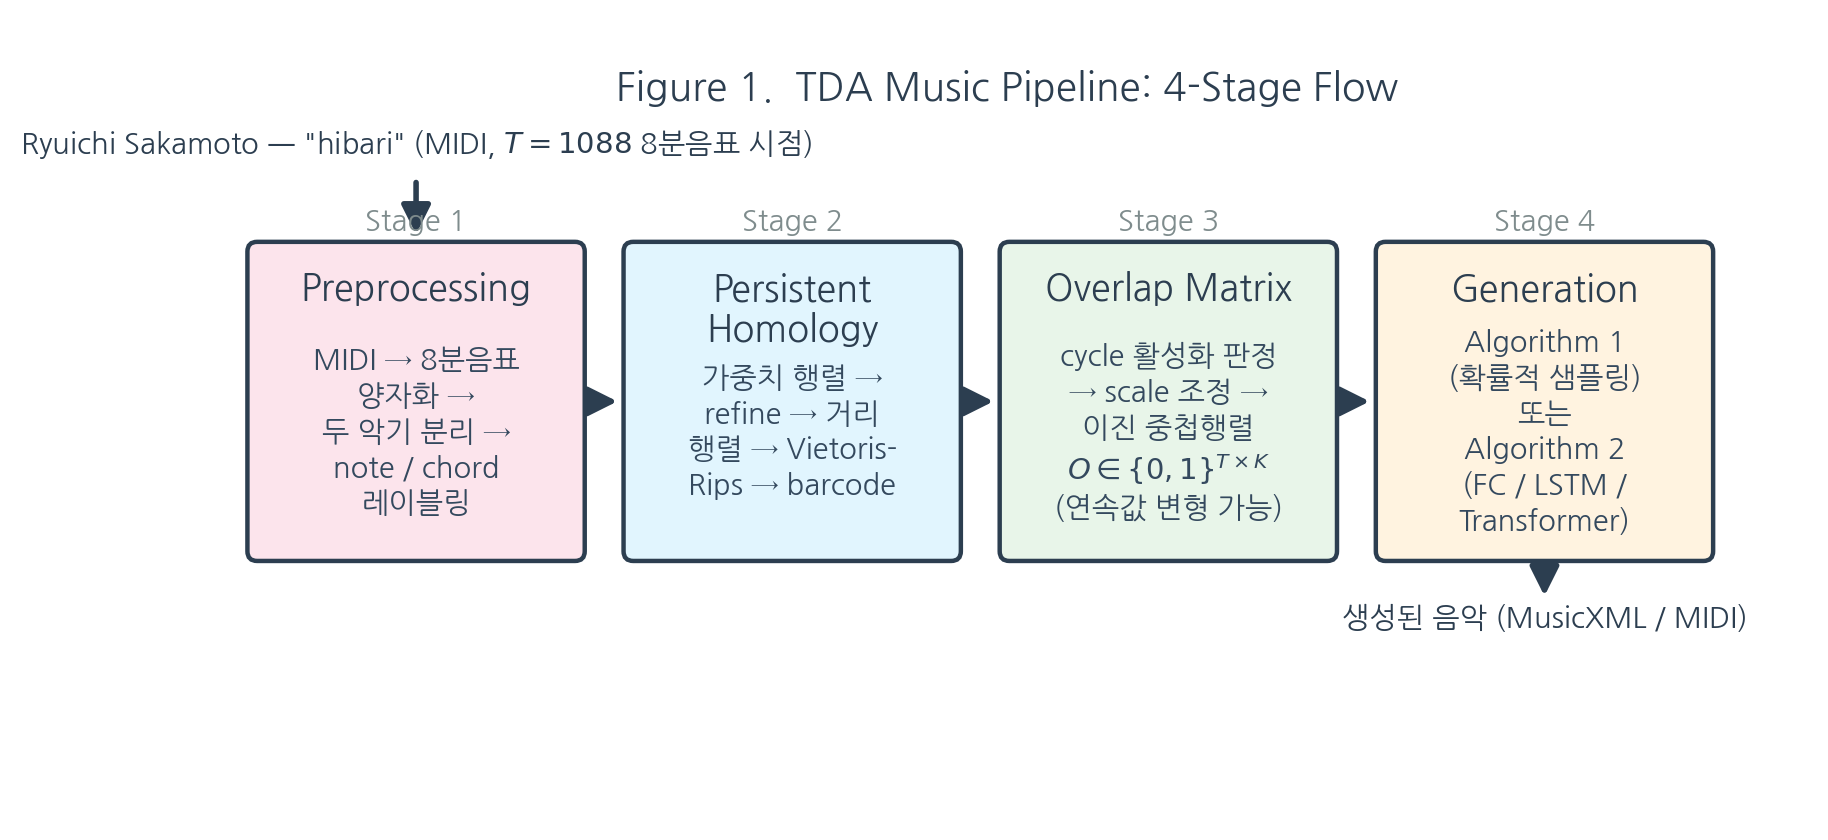
\includegraphics[width=0.9\textwidth]{fig1_pipeline.png}
\caption{4단계 파이프라인: (1)~MIDI 전처리, (2)~persistent homology,
(3)~중첩행렬 구축, (4)~Algorithm~1 또는~2에 의한 생성.}
\label{fig:pipeline}
\end{figure}

\subsection{1단계: 전처리}
MIDI 파일을 8분음표 단위로 양자화하고 ($T = 1{,}088$), 두 악기를
분리하며, 각 고유 (pitch, duration) 쌍에 1-indexed 레이블을 부여한다
(\emph{hibari}: $N = 23$ note, $C = 17$ 화음).

\subsection{2단계: Persistent Homology}
가중 note 네트워크를 구성하고 (\S\ref{subsec:weights}),
거리 행렬을 유도하여 $r \in [0, 1.5]$에 걸친 $H_1$ filtration을
계산한다.

\subsection{3단계: 중첩행렬}
모든 시점에서 cycle 활성화를 계산하고 임계값을 적용한다
(\S\ref{subsec:overlap}).

\subsection{Algorithm 1 --- 위상적 샘플링}
\label{subsec:algo1}

각 시점 $t$에 대해:
\begin{itemize}
\item 활성 cycle이 존재하면 ($\sum_c O[t,c] > 0$): \emph{교집합}
      $I(t) = \bigcap_{c: O[t,c]=1} V(c)$에서 샘플링.
      $I(t) = \emptyset$이면 합집합 $U(t)$로 대체.
\item 활성 cycle이 없으면: 인접 활성 cycle vertex의 여집합
      $P \setminus A(t)$에서 샘플링 (위상적 ``번짐'' 방지).
\item 충돌 회피: 시점당 최대 $R = 50$회 재샘플링.
\end{itemize}

\subsection{Algorithm 2 --- 신경망 시퀀스 모델}
\label{subsec:algo2}

매핑 $f_\theta : O[t,:] \mapsto y[t,:]$을 학습하는 세 가지
아키텍처:
\begin{itemize}
\item \textbf{FC}: 2층 완전연결 ($H = 128$), 시점 독립.
\item \textbf{LSTM}: 2층, 순방향 시퀀스 문맥.
\item \textbf{Transformer}: 2층, 4-head, 학습 가능 위치 임베딩.
\end{itemize}

모든 모델은 \texttt{BCEWithLogitsLoss}와 데이터 증강(부분집합 샘플링,
순환 이동, 비트 플립 노이즈)을 사용한다. 추론 시 적응형 임계값
$\theta = \mathrm{quantile}(P, 1-\rho_{\mathrm{on}})$으로
원곡 ON 비율 $\rho_{\mathrm{on}} \approx 0.15$를 맞춘다.


% ═════════════════════════════════════════════════════════════════════════
% §4 실험
% ═════════════════════════════════════════════════════════════════════════
\section{실험}
\label{sec:experiments}

모든 실험은 $N = 20$회 독립 반복으로 수행하였다. 주요 지표는
pitch JS divergence이다.

\subsection{거리 함수 비교}
\label{subsec:dist_compare}

\begin{table}[H]
\centering
\caption{네 가지 거리 함수에 대한 Algorithm~1 JS divergence
($N = 20$, 감쇄 lag $\ell \in \{1,\ldots,4\}$).}
\label{tab:baselines}
\begin{tabular}{lccc}
\toprule
거리 함수 & $K$ & JS (평균 $\pm$ 표준편차) & Coverage \\
\midrule
frequency      & 43 & $0.0753 \pm 0.0033$ & $0.991$ \\
\textbf{Tonnetz} & \textbf{46} & $\mathbf{0.0398 \pm 0.0031}$ & $1.000$ \\
voice-leading  & 22 & $0.0891 \pm 0.0048$ & $1.000$ \\
DFT            & 20 & $0.0511 \pm 0.0029$ & $1.000$ \\
\bottomrule
\end{tabular}
\end{table}

Tonnetz는 frequency 대비 JS를 $47\%$ 감소시킨다 (표~\ref{tab:baselines}).
Welch $t = 35.1$, $\nu \approx 38$, $p < 10^{-20}$, Cohen's $d = 11.1$.

\subsection{옥타브 가중치 튜닝}
\label{subsec:octave}

$w_o \in \{0.1, 0.3, 0.5, 0.7, 1.0\}$에 대한 격자 탐색 ($N = 10$)
결과, $w_o = 0.3$이 최적이다 (JS $0.0479$, $w_o = 0.5$ 대비 $-18.8\%$).
\emph{hibari}의 좁은 2옥타브 음역(MIDI 52--81)과 일치한다.

\subsection{Cycle 부분집합 절제}

\begin{table}[H]
\centering
\caption{Cycle 부분집합 절제 (Tonnetz, $N=20$).}
\label{tab:ablation}
\begin{tabular}{ccc}
\toprule
$K$ & JS (평균 $\pm$ 표준편차) & Coverage \\
\midrule
10  & $0.0991 \pm 0.0038$ & $0.980$ \\
17  & $0.0740 \pm 0.0038$ & $0.996$ \\
46  & $\mathbf{0.0397 \pm 0.0025}$ & $1.000$ \\
\bottomrule
\end{tabular}
\end{table}

JS는 $K$에 대해 단조 감소하지만 수확 체감이 나타난다
(표~\ref{tab:ablation}).

\subsection{연속값 중첩행렬}
\label{subsec:continuous}

\begin{table}[H]
\centering
\caption{연속값 중첩행렬 실험 (Tonnetz, $N=20$).}
\label{tab:continuous}
\begin{tabular}{lcc}
\toprule
설정 & Density & JS (평균 $\pm$ 표준편차) \\
\midrule
이진 (캐시)                & $0.751$ & $0.0387 \pm 0.0027$ \\
연속값 직접 사용            & $0.264$ & $0.0382 \pm 0.0021$ \\
연속 $\to$ 이진 $\tau{=}0.3$ & $0.373$ & $0.0386 \pm 0.0022$ \\
\textbf{연속 $\to$ 이진 $\tau{=}0.5$} & $\mathbf{0.168}$ & $\mathbf{0.0343 \pm 0.0027}$ \\
연속 $\to$ 이진 $\tau{=}0.7$ & $0.077$ & $0.0364 \pm 0.0032$ \\
\bottomrule
\end{tabular}
\end{table}

연속값 중첩행렬에 $\tau = 0.5$ 이진화를 적용하면 이진 기준선 대비
$11.4\%$ 추가 개선된다 (Welch $t = 5.16$, $p < 0.001$, $d = 1.63$;
표~\ref{tab:continuous}).

\subsection{심층학습 모델 비교}
\label{subsec:dl}

\begin{table}[H]
\centering
\caption{최적 DL 설정 (각 1회 실행).}
\label{tab:dl}
\begin{tabular}{lccc}
\toprule
모델 & Val Loss & JS & 생성 Note 수 \\
\midrule
FC (hd=256, do=0.3)   & $0.282$ & $\mathbf{0.0015}$ & $3{,}754$ \\
LSTM (2층)              & $0.385$ & $0.0448$ & $3{,}753$ \\
Transformer (2L, 4H)   & $0.676$ & $0.0104$ & $3{,}753$ \\
\bottomrule
\end{tabular}
\end{table}

가장 단순한 FC 모델이 최저 JS를 달성한다 (표~\ref{tab:dl}).
이는 \emph{hibari}의 미학을 반영한다: \emph{out of noise}는
시간적 인과보다 음의 공간적 배치를 중시하므로, 시간 문맥을
무시하는 FC가 작곡 설계와 더 잘 부합한다.

\subsection{개선 F: 연속값 중첩행렬 + FC}
\label{subsec:improvF}

\begin{table}[H]
\centering
\caption{FC에 대한 연속 vs.\ 이진 입력 ($N=5$).}
\label{tab:improvF}
\begin{tabular}{lcccc}
\toprule
입력 & JS (평균 $\pm$ 표준편차) & Val Loss & Coverage \\
\midrule
이진      & $0.0014 \pm 0.0010$ & $0.070$ & $0.948$ \\
\textbf{연속} & $\mathbf{0.0006 \pm 0.0005}$ & $\mathbf{0.031}$ & $\mathbf{0.991}$ \\
\bottomrule
\end{tabular}
\end{table}

연속 입력은 JS를 $57\%$, val loss를 $2.3$배 감소시킨다
(표~\ref{tab:improvF}). 본 연구에서 관측된 최저 전곡 JS이다
(이론적 최댓값 $\log 2$의 $0.09\%$).

\subsection{곡 고유 구조 분석}
\label{subsec:structure}

\paragraph{Deep scale 특성}
\emph{hibari}의 7개 pitch class $\{C, D, E, F, G, A, B\}$는
음정 벡터 $[2,5,4,3,6,1]$을 가지며, 모든 성분이 상이하다.
이는 온음계 고유의 특성이다 \cite{gamer2003}.

\paragraph{준균등 pitch 분포}
\label{subsec:phase}
정규화 pitch 엔트로피가 $0.974$ (거의 최대)이다.
모든 pitch가 거의 동일 확률로 나타나므로, 시간 순서를 무시하는 FC가
이미 참 분포를 잘 근사함을 설명한다.

\paragraph{Tonnetz 판별력}
7개 PC에서 Tonnetz 직경은 $4$로, 세밀한 거리 판별이 가능하다.
12개 PC(\emph{solari} 등)에서는 직경이 $2$로 축소되어
Tonnetz의 이점이 사라진다.

\paragraph{위상 이동(Phase shifting)}
악기~1은 32-step 모듈을 $33$회 반복(쉼 없음);
악기~2는 33-step 모듈을 $32$회 반복(모듈당 쉼 1회).
서로소 주기 ($\gcd(32,33) = 1$)에 의해 두 악기는 결코 동기화되지
않는다. Steve Reich의 \emph{phase shifting} 기법과 수학적으로 동일한
구조이다.


% ═════════════════════════════════════════════════════════════════════════
% §5 시각자료
% ═════════════════════════════════════════════════════════════════════════
\section{시각자료}
\label{sec:figures}

6개의 정적 도표와 1개의 대화형 HTML 보충자료를 제공한다.

\begin{figure}[H]
\centering
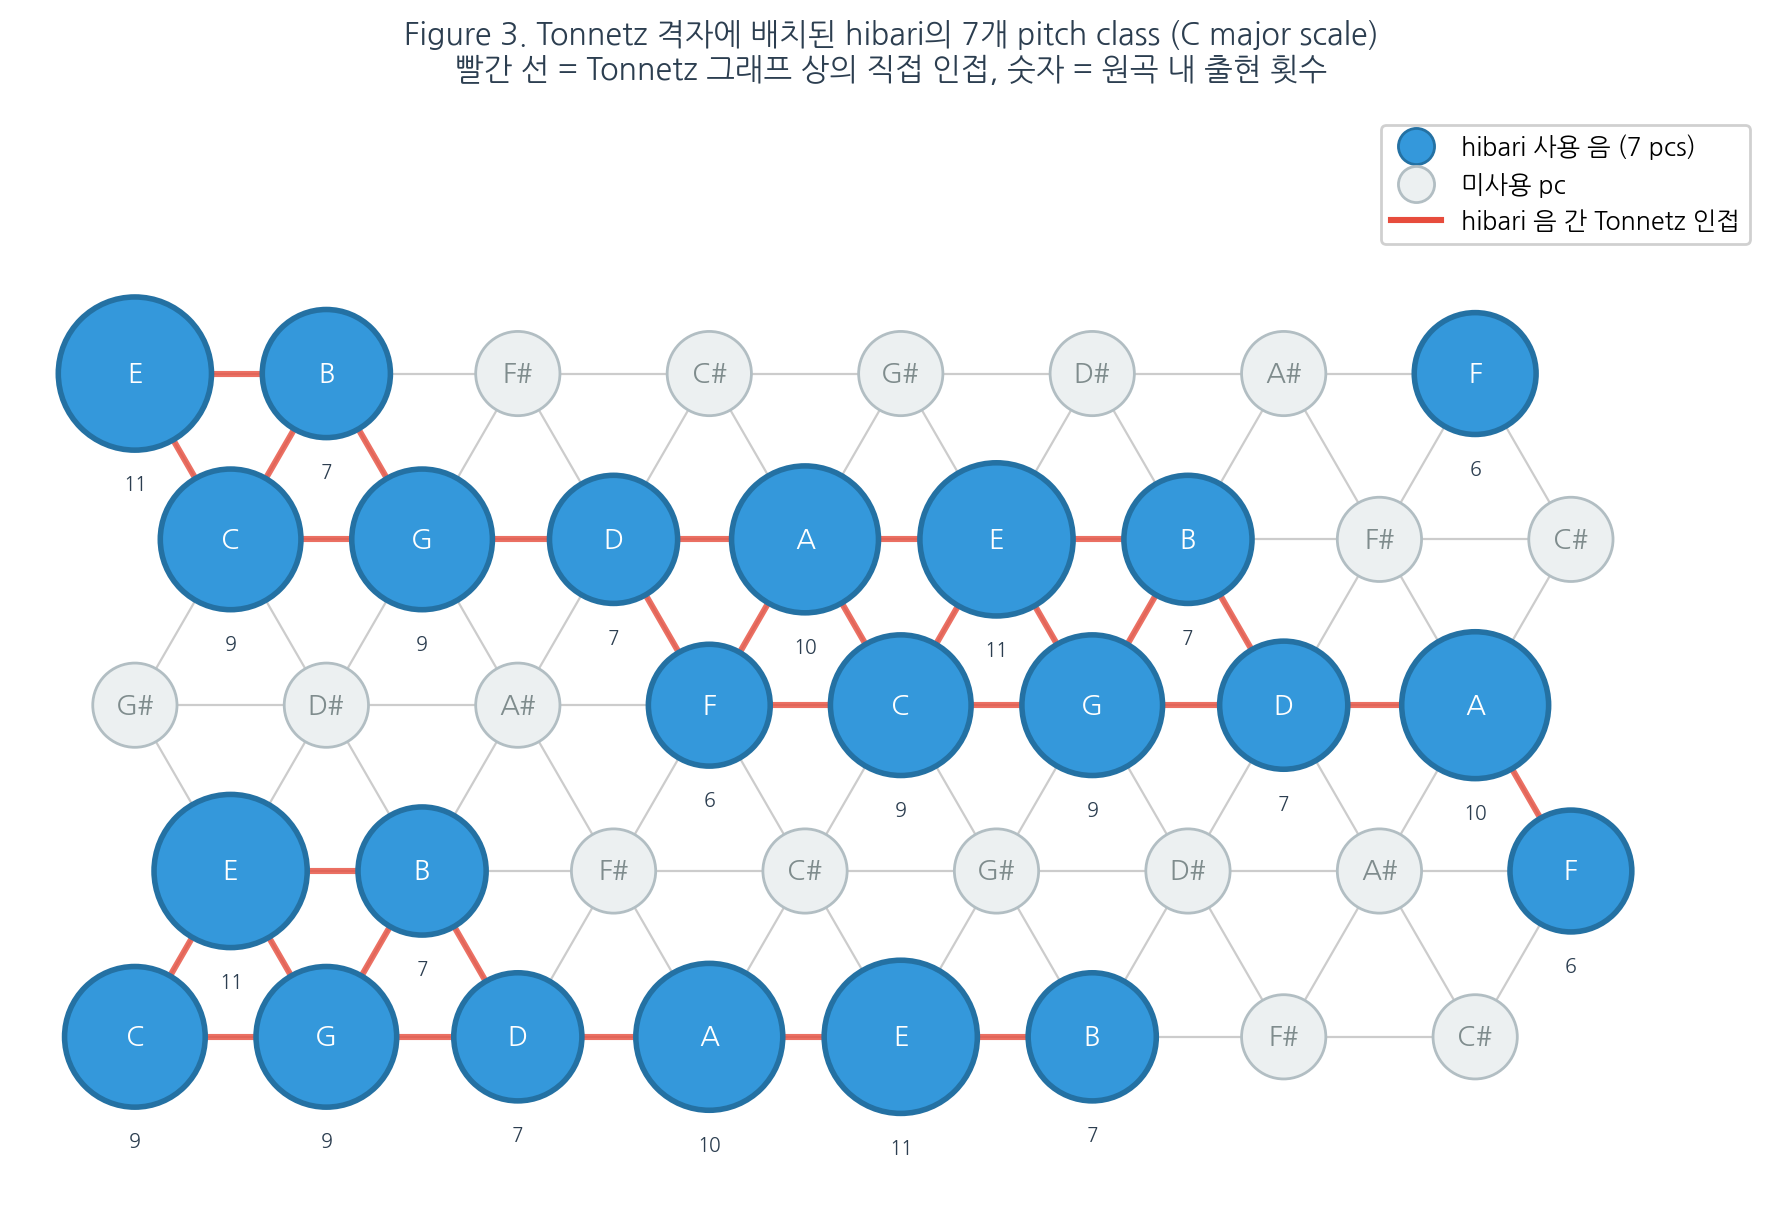
\includegraphics[width=0.75\textwidth]{fig3_tonnetz_hibari.png}
\caption{Tonnetz 격자 위의 \emph{hibari} 7개 pitch class (파란색).
빨간 간선은 직접 Tonnetz 인접을 나타낸다.}
\label{fig:tonnetz}
\end{figure}

\begin{figure}[H]
\centering
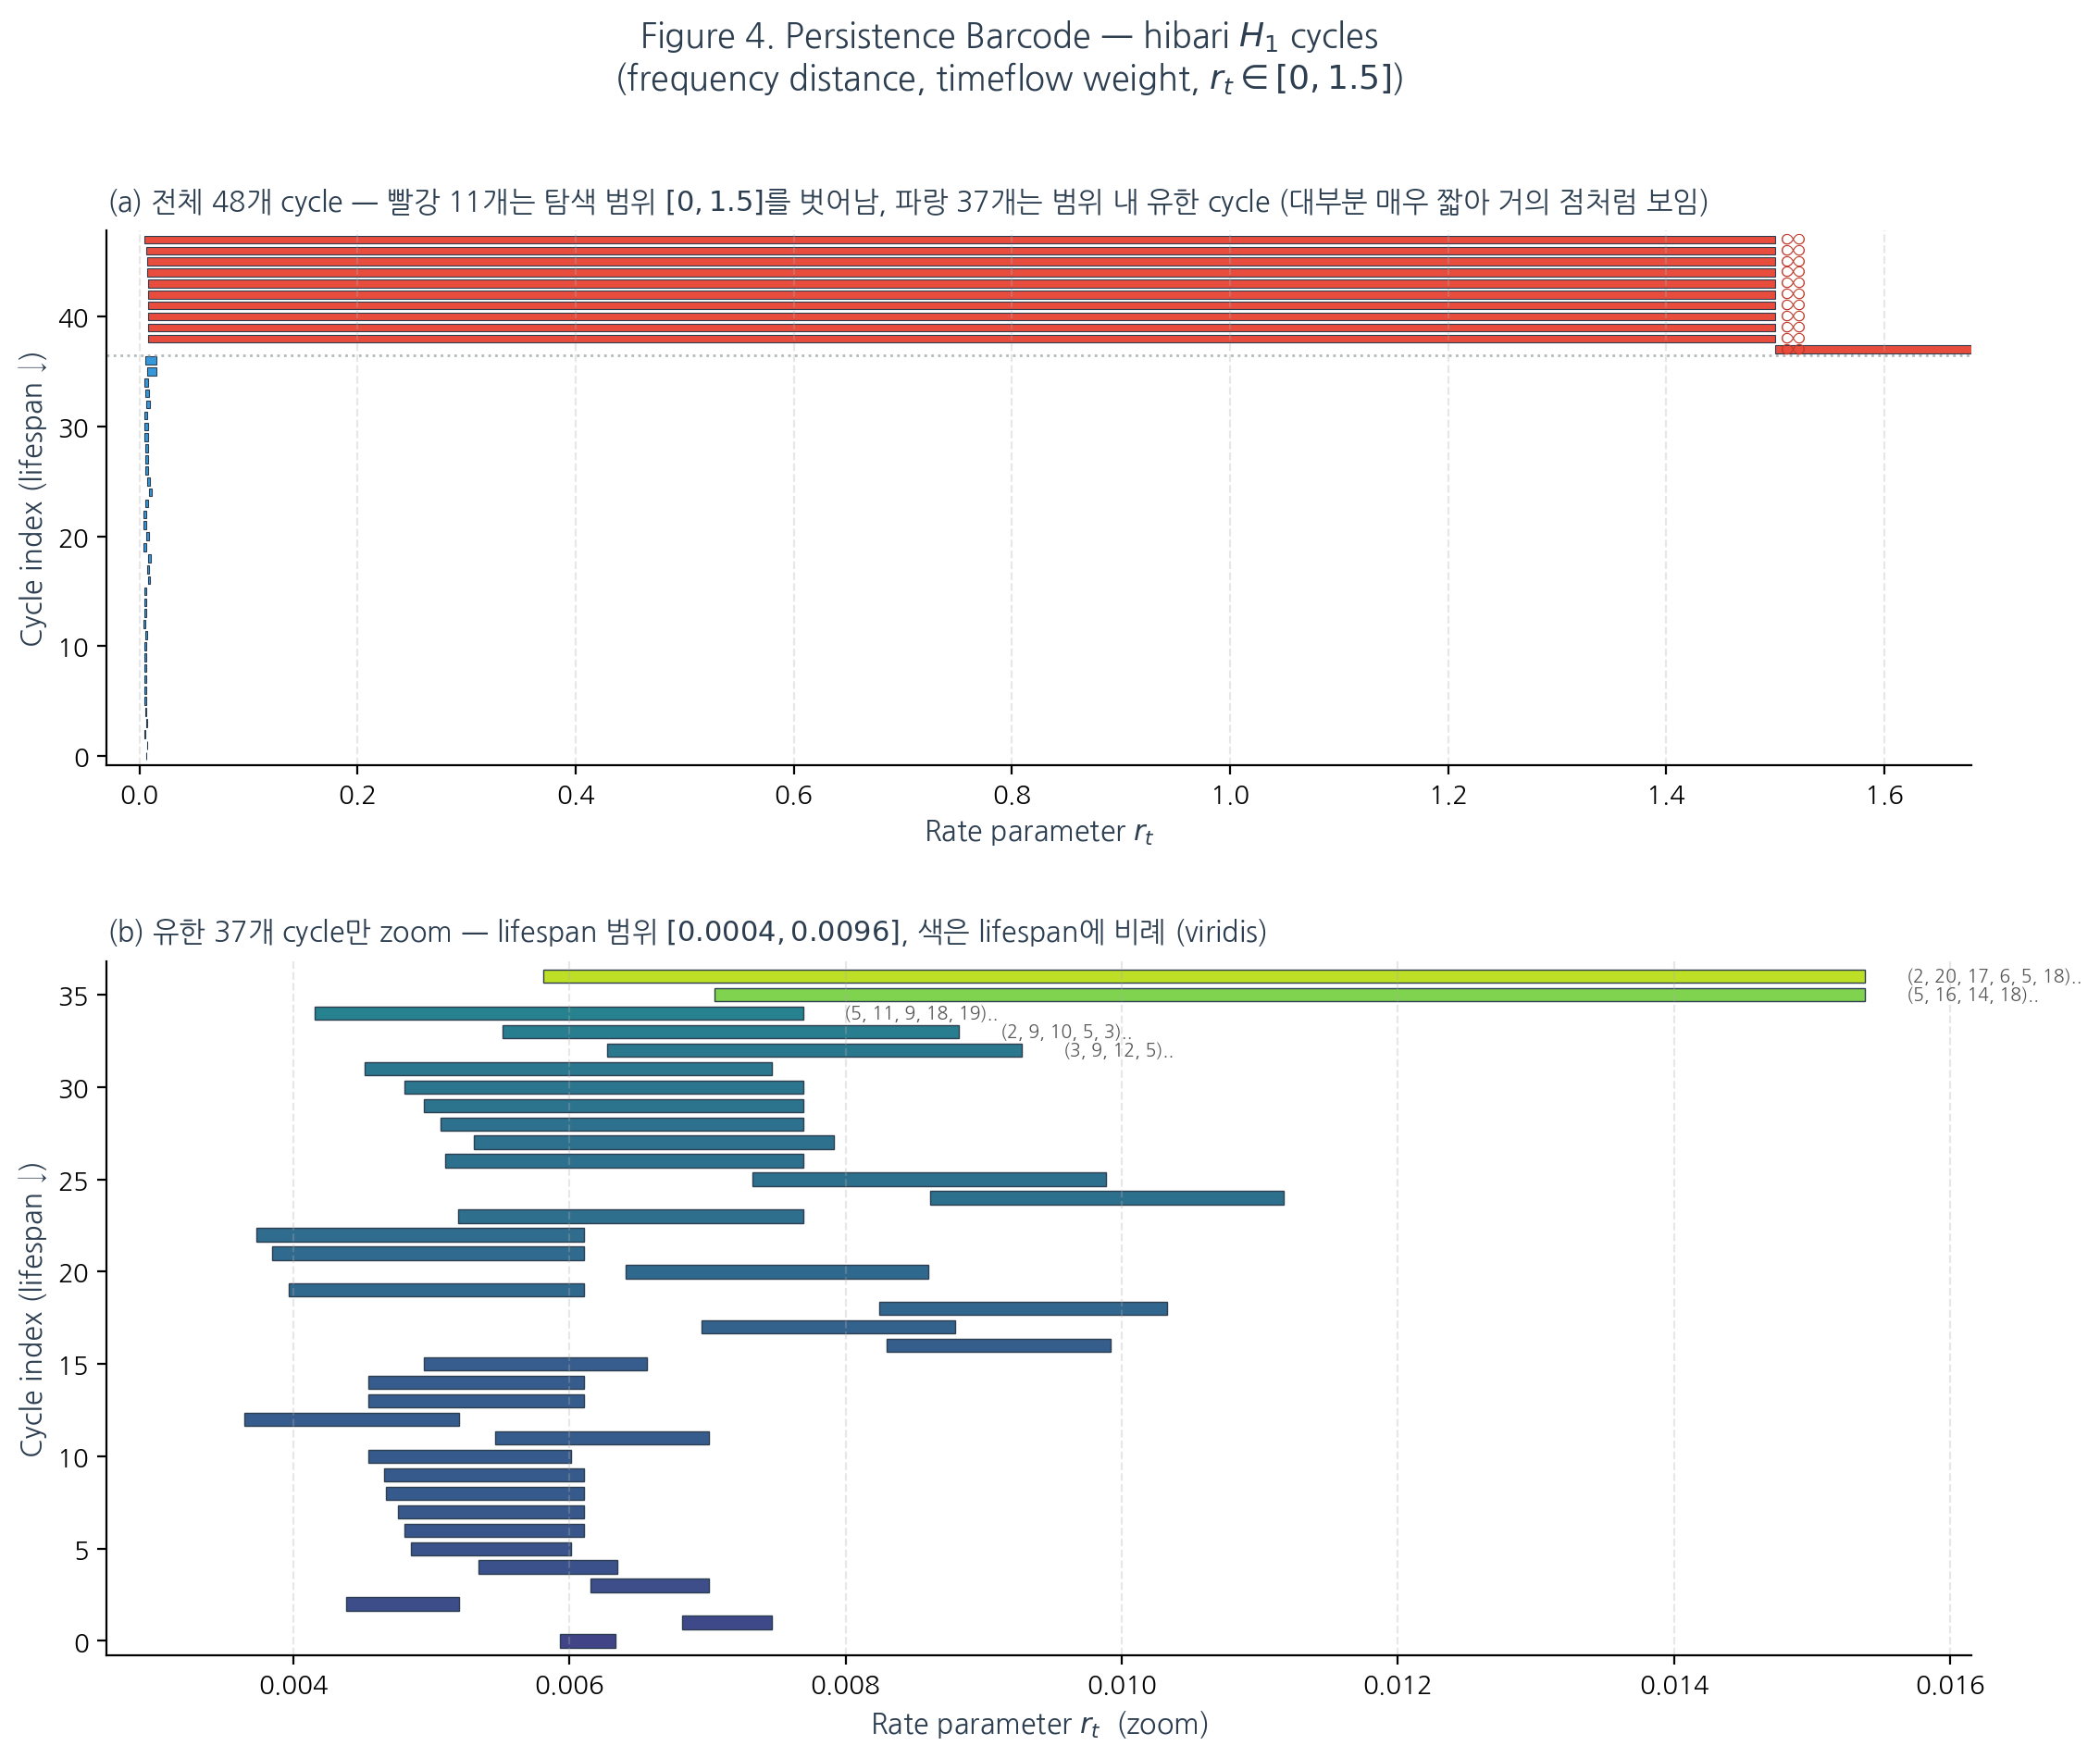
\includegraphics[width=0.85\textwidth]{fig4_barcode.png}
\caption{$H_1$ persistence barcode (Tonnetz). 위: 전체 barcode;
아래: 유한 cycle 확대. 수명 범위가 $10{,}000$배 이상 차이난다.}
\label{fig:barcode}
\end{figure}

\begin{figure}[H]
\centering
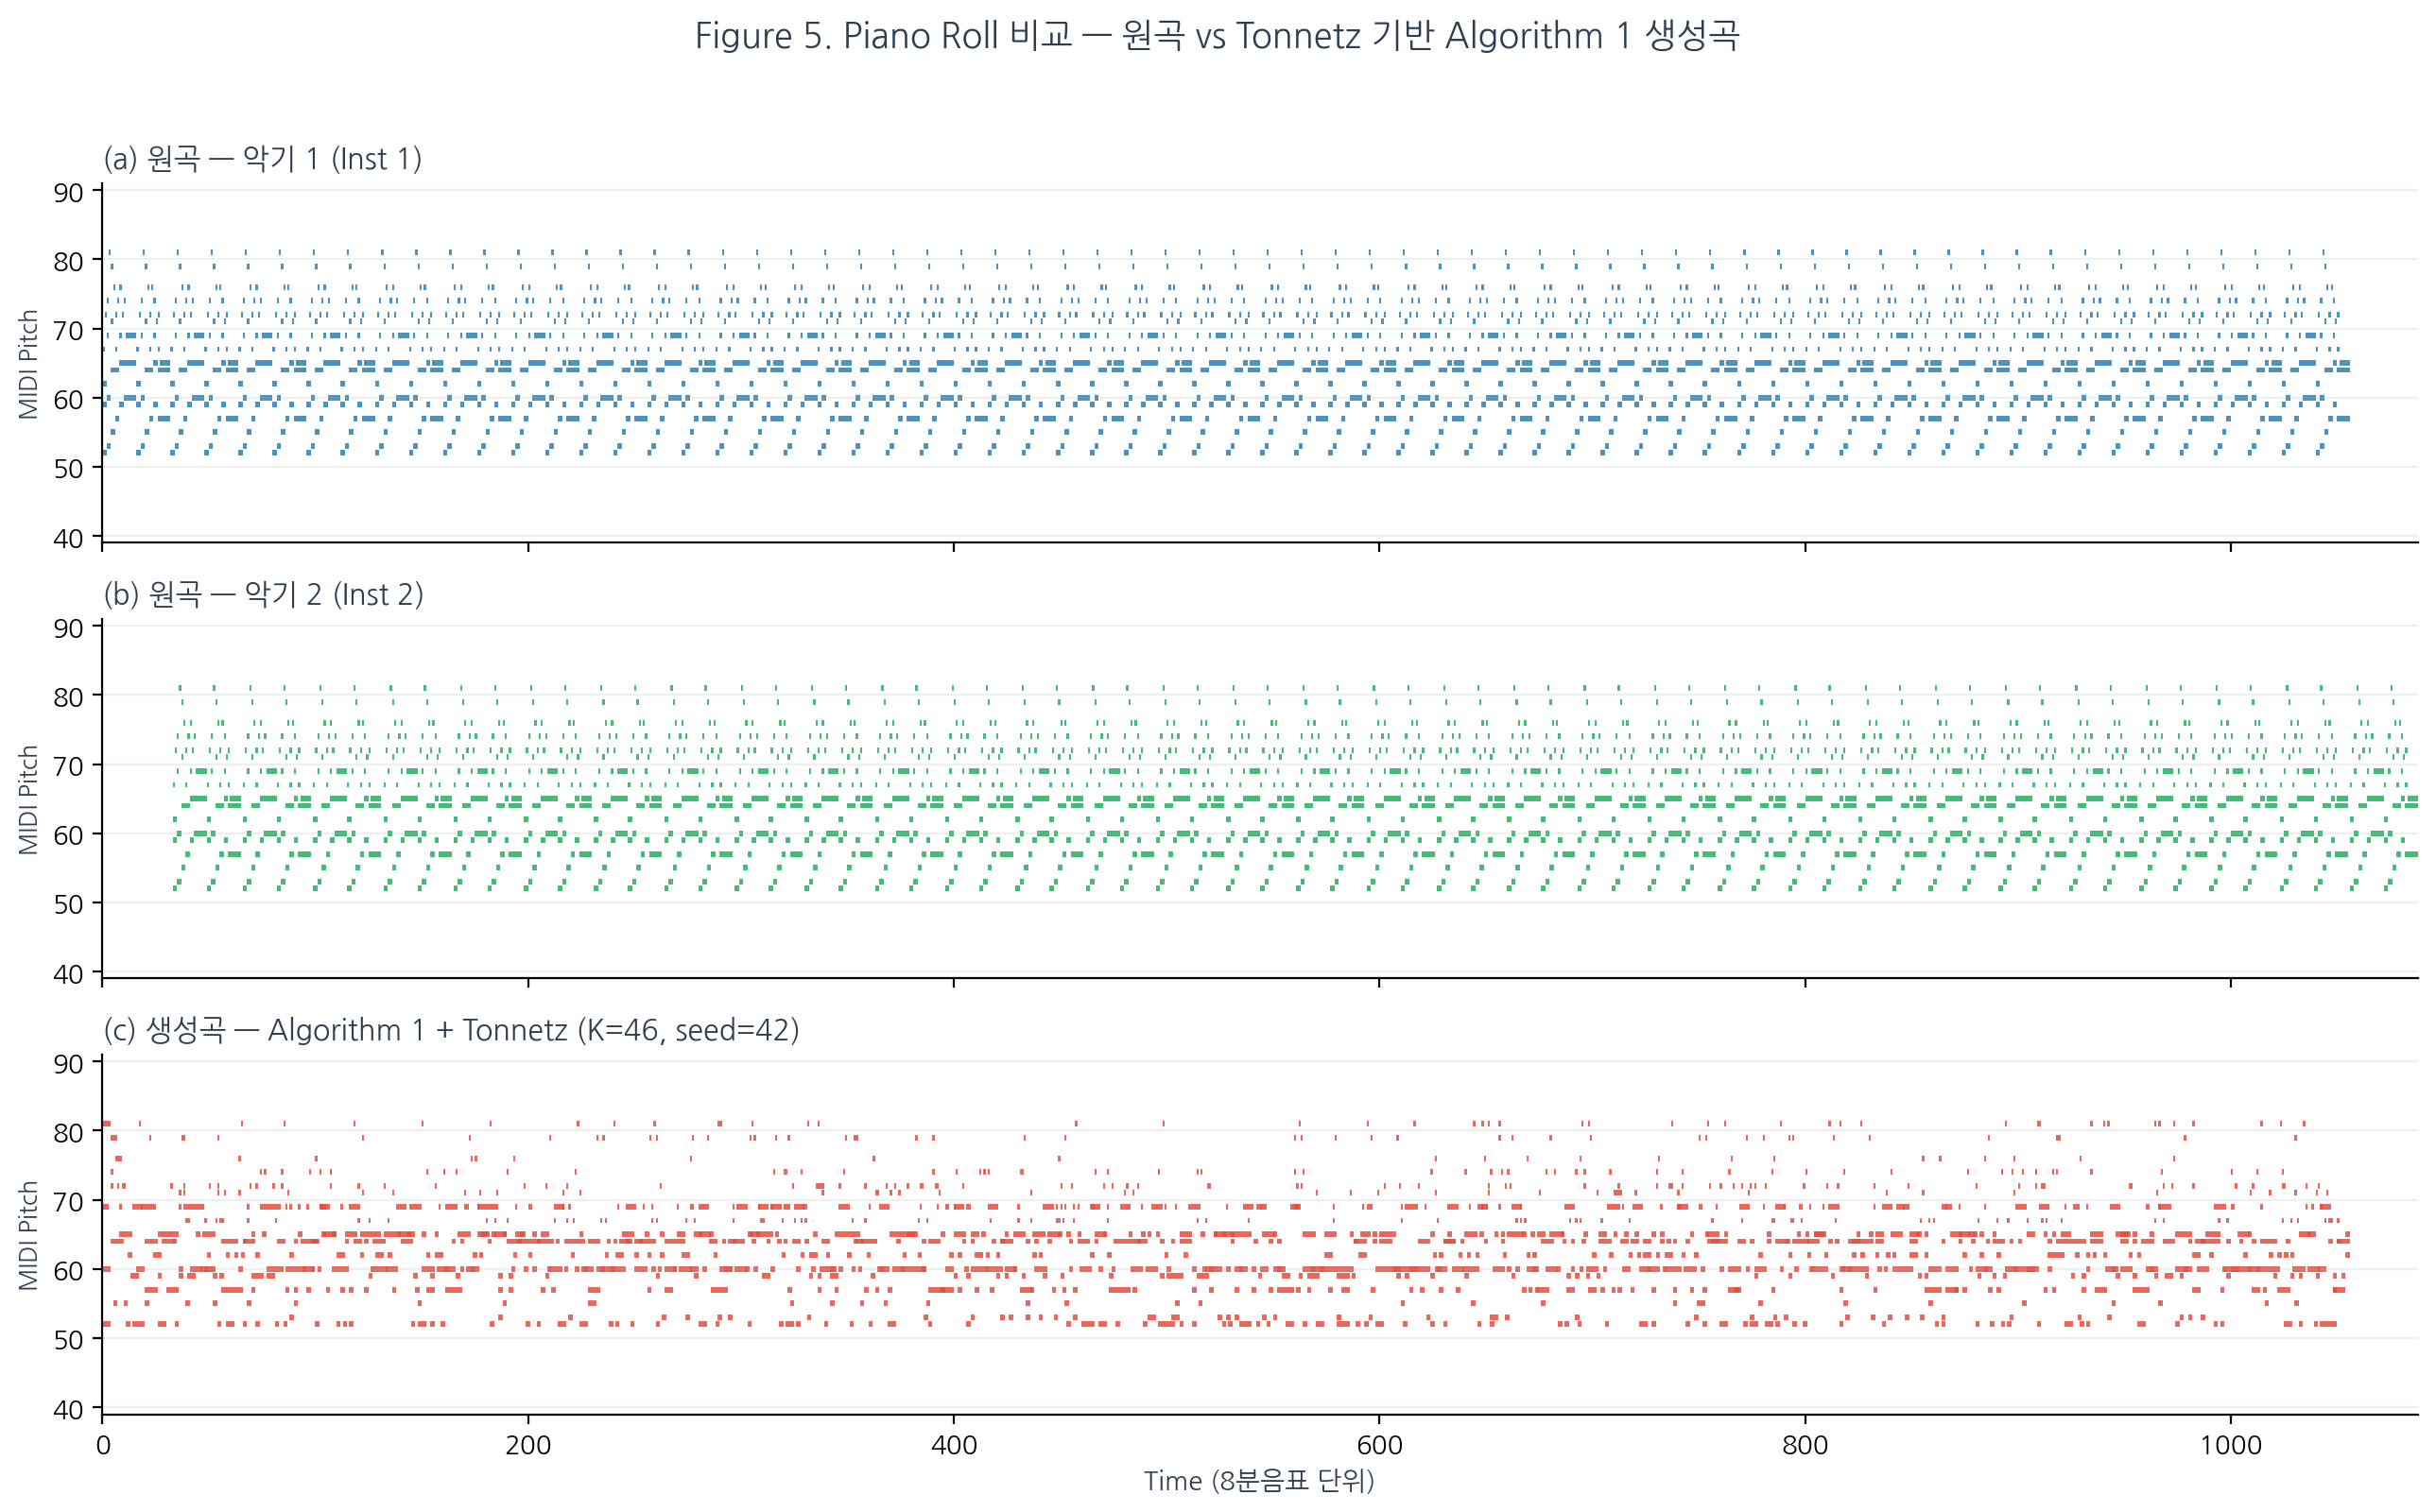
\includegraphics[width=0.85\textwidth]{fig5_pianoroll.png}
\caption{피아노 롤 비교: (a)--(b) 원곡 악기 1--2;
(c)~Algorithm~1 + Tonnetz.}
\label{fig:pianoroll}
\end{figure}

\begin{figure}[H]
\centering
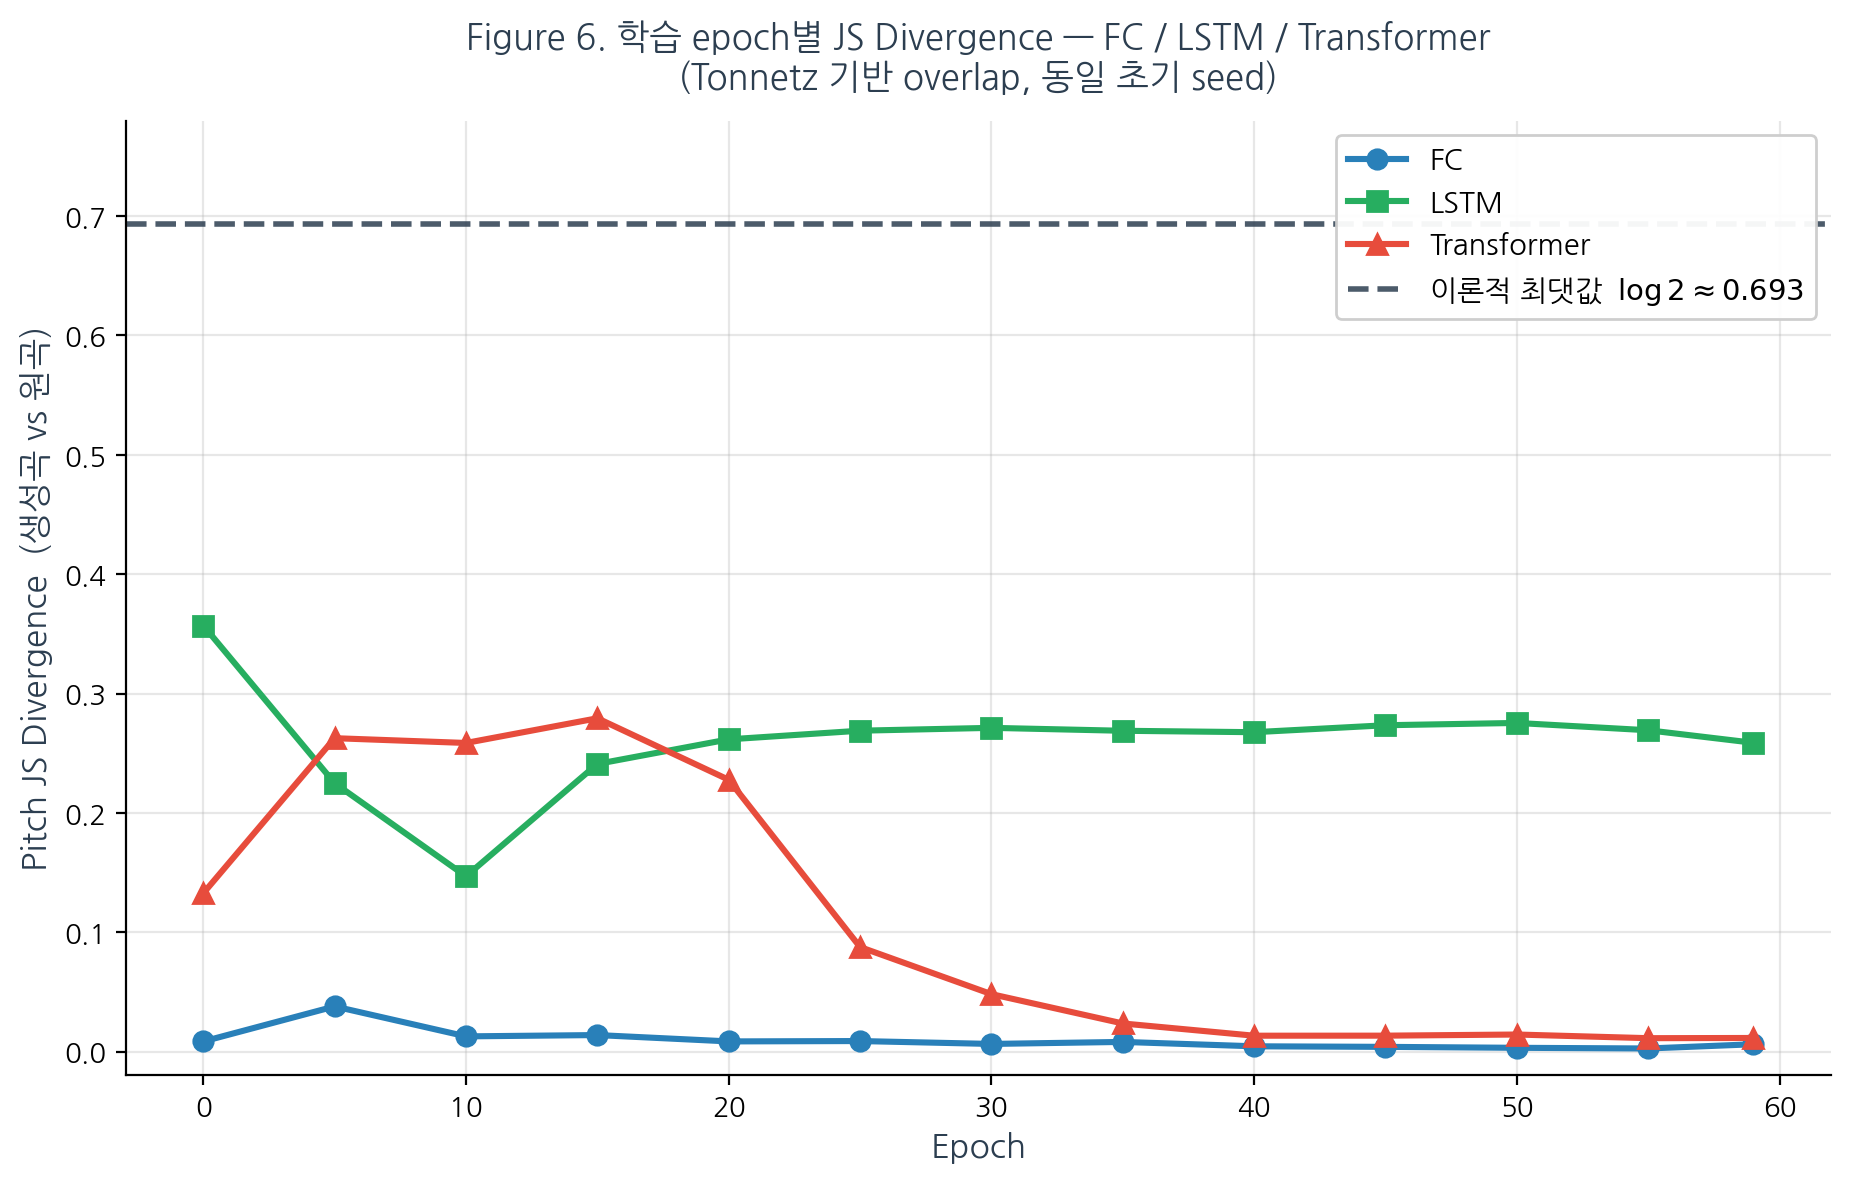
\includegraphics[width=0.75\textwidth]{fig6_js_curve.png}
\caption{학습 epoch에 따른 JS divergence. FC가 가장 빠르게 수렴;
LSTM은 $\mathrm{JS} \approx 0.26$에서 정체.}
\label{fig:jscurve}
\end{figure}


% ═════════════════════════════════════════════════════════════════════════
% §6 차별화
% ═════════════════════════════════════════════════════════════════════════
\section{관련 연구와의 비교}
\label{sec:differentiation}

\subsection{일반 AI 음악 생성과의 비교}

코퍼스 기반 학습 모델(Magenta, Music Transformer)과 달리,
본 파이프라인은 \emph{단일 곡에 대한 심층 분석}을 수행하여
해석 가능하고 추적 가능한 생성을 실현한다.
FC~$>$~Transformer라는 결과는 ``더 많은 시간적 모델링이 항상
우월하다''는 보편적 가정에 도전한다.

\subsection{기존 TDA--음악 연구와의 비교}

선행 TDA--음악 연구 \cite{tran2021,lee2024}와 비교하여:
\begin{enumerate}[label=(\Alph*)]
\item 네 가지 거리 함수를 $N{=}20$ 통계로 체계적 비교.
\item 연속값 중첩행렬 도입.
\item 완전한 통계적 엄밀성 (Welch $t$, Cohen's $d$) 제공.
\item 서양 현대음악으로 확장.
\item 모델 선택과 미학적 맥락의 연결.
\item TDA를 분석에서 \emph{변주}로 확장 (\S\ref{sec:extensions}).
\end{enumerate}


% ═════════════════════════════════════════════════════════════════════════
% §7 확장 실험
% ═════════════════════════════════════════════════════════════════════════
\section{확장 실험}
\label{sec:extensions}

\subsection{모듈 단위 생성}
\label{subsec:module}

\emph{hibari}의 32-step 모듈 구조에 착안하여, 단일 모듈을 생성한 후
$33$회 복제하는 방법을 탐구하였다.
5가지 프로토타입 전략을 비교하였으며,
P4(첫 모듈의 국소 PH, $K{=}24$ cycle)와 best-of-10 선택(C)의
결합이 최적이었다:

\begin{table}[H]
\centering
\caption{모듈 단위 생성 전략 ($N=10$).}
\label{tab:module}
\begin{tabular}{lcccc}
\toprule
전략 & JS (평균$\pm$표준편차) & 최저 & Cov. \\
\midrule
P1 기준선        & $0.114 \pm 0.039$ & $0.074$ & $0.77$ \\
C: best-of-10   & $0.074 \pm 0.027$ & $0.024$ & $0.90$ \\
D: cov$\ge$20/23 & $0.082 \pm 0.022$ & $0.050$ & $0.88$ \\
P4: 국소 PH      & $0.066 \pm 0.019$ & $0.038$ & $0.84$ \\
\textbf{P4+C}    & $\mathbf{0.059 \pm 0.015}$ & $\mathbf{0.026}$ & $0.89$ \\
\bottomrule
\end{tabular}
\end{table}

8개 시작 위치에 대한 분석 결과 모듈~0 ($t \in [0,32)$)이 최적이다
(JS~$0.054$, 최저~$0.026$). 최적 단일 시행(seed~9302, JS~$= 0.0258$)은
전곡 기준선 평균($0.0398$)을 능가한다.

\subsection{일반화: \emph{solari}, Bach, Ravel}
\label{subsec:generalization}

\begin{table}[H]
\centering
\caption{교차 곡 비교 요약.}
\label{tab:generalization}
\begin{tabular}{lcccc}
\toprule
곡 & PC 수 & 최적 거리 & 최적 모델 & 해석 \\
\midrule
hibari & 7 & Tonnetz & FC & 공간적 배치 \\
solari & 12 & freq/Ton. & Transformer & 선율적 진행 \\
aqua   & 12 & Tonnetz & --- & Tonnetz $+26.3\%$ \\
Bach   & 12 & Tonnetz & --- & Tonnetz $-54.8\%$ \\
Ravel  & 12 & frequency & FC & 풍부한 분포 \\
\bottomrule
\end{tabular}
\end{table}

\emph{solari} (12-PC, 반음계)에서는 Transformer가 최적이다
(JS~$0.016$). \emph{hibari}의 FC 우위와 정확히 역전된다
(표~\ref{tab:generalization}).
Bach Fugue에서 Tonnetz는 $-54.8\%$로 관측 중 최대 개선을 보이고,
Ravel Pavane ($N{=}49$ note)에서는 frequency가 최적이다.

\subsection{방향 A: 위상 보존 Note 재분배}
\label{subsec:dirA}

Cycle vertex 집합을 Tonnetz 매칭 거리가 최소화되는 새 note로
교체한다. 중첩행렬은 그대로 보존된다.

\begin{table}[H]
\centering
\caption{Note 재분배 (Algorithm~1, Tonnetz).}
\label{tab:redistrib}
\begin{tabular}{lcccc}
\toprule
설정 & Note 오차 & Cycle 오차 & DTW & $\Delta$DTW \\
\midrule
기준선     & --- & --- & $2.21$ & --- \\
narrow    & $4.00$ & $1.17$ & $2.09$ & $-5.8\%$ \\
wide      & $4.46$ & $1.18$ & $2.89$ & $+30.3\%$ \\
\textbf{vwide} & $4.48$ & $1.06$ & $\mathbf{3.57}$ & $\mathbf{+61.4\%}$ \\
\bottomrule
\end{tabular}
\end{table}

가장 넓은 음역(MIDI 40--88)에서 DTW가 $61.4\%$ 증가하면서도
cycle 오차는 $\sim 1.1$로 안정적이다 (표~\ref{tab:redistrib}) ---
위상 구조를 보존하면서 멜로디가 실질적으로 다른 음악이 생성된다.

\subsection{방향 B: 시간 재배치}
\label{subsec:dirB}

세 가지 전략(구간 셔플, 블록 순열, Markov 재샘플링)을 시험하였다.
PE 제거 및 재학습을 적용한 Transformer가 DTW~$+21.7\%$를 달성하나,
pitch JS가 $0.007 \to 0.173$으로 악화된다.
방향~B 단독으로는 pitch 분포 보존과 멜로디 변화를 동시에 달성할 수 없으며,
방향~A와의 결합이 필요하다.

\subsection{화성 제약}
\label{subsec:harmony}

Note 재분배에 음계 제약(major, minor, pentatonic)과 협화 목표를
추가하였다. \textbf{scale\_major}가 가장 효과적이다:
note 오차 $4.35 \to 3.52$ ($-19\%$), 음계 일치 $1.00$,
평균 불협화도 $0.412 \to 0.361$.

\subsection{A+B 결합: 최종 통합}
\label{subsec:combined_ab}

최적 결합 설정 (\textbf{major\_block32}):
scale\_major 재분배 + 블록 순열(32) + 연속 중첩행렬 + Transformer.
결과: ref~pJS $= 0.002$ (거의 완벽한 학습),
DTW $+31\%$ (다른 멜로디),
C~major 음계 일치 $= 1.00$.

\subsection{Cycle별 임계값 최적화}
\label{subsec:percycle}

각 cycle에 대해 $\tau_c \in \{0.1, 0.2, \ldots, 0.7\}$로
탐욕적 좌표 하강법을 수행하였다:

\begin{table}[H]
\centering
\caption{Cycle별 $\tau_c$ 최적화 ($N=20$).}
\label{tab:percycle}
\begin{tabular}{lcc}
\toprule
설정 & JS (평균 $\pm$ 표준편차) & 개선율 \\
\midrule
균일 $\tau = 0.35$ & $0.0460 \pm 0.0034$ & --- \\
\textbf{Cycle별 $\tau_c$} & $\mathbf{0.0241 \pm 0.0023}$ & $\mathbf{+47.5\%}$ \\
\bottomrule
\end{tabular}
\end{table}

$47.5\%$ 개선 ($p < 0.001$; 표~\ref{tab:percycle}). 대다수 cycle이
$\tau < 0.35$를 선호하여, 기존에 ``반주형'' cycle이 억제되고 있었음을
시사한다. 과적합 없음: N=5 탐색 결과($0.0238$)가
N=20 검증($0.0241$)과 일치.

\subsection{Soft Activation: 전체 아키텍처}
\label{subsec:soft}

\begin{table}[H]
\centering
\caption{이진 vs.\ 연속 입력 ($N=5$).}
\label{tab:soft}
\begin{tabular}{llccc}
\toprule
모델 & 입력 & JS & Val Loss & $\Delta$JS \\
\midrule
FC   & 이진 & $0.0035$ & $0.307$ & --- \\
\textbf{FC} & \textbf{연속} & $\mathbf{0.0004}$ & $\mathbf{0.026}$ & $\mathbf{+88.6\%}$ \\
Trans. & 이진 & $0.0034$ & $0.465$ & --- \\
\textbf{Trans.} & \textbf{연속} & $\mathbf{0.0007}$ & $\mathbf{0.121}$ & $\mathbf{+79.4\%}$ \\
LSTM & 이진 & $0.280$ & $0.411$ & --- \\
LSTM & 연속 & $0.290$ & $0.411$ & $-3.5\%$ \\
\bottomrule
\end{tabular}
\end{table}

FC와 Transformer는 연속 입력으로 대폭 개선되나,
LSTM은 호환되지 않는다 (표~\ref{tab:soft}).
FC + 연속 입력이 JS~$= 0.0004$로 본 연구 전체 최저치이다.

\subsection{Tonnetz $\alpha$ 격자 탐색}
\label{subsec:alpha}

\begin{table}[H]
\centering
\caption{$\alpha$ 격자 탐색 ($N=20$).}
\label{tab:alpha}
\begin{tabular}{cccc}
\toprule
$\alpha$ & $K$ & JS (평균 $\pm$ 표준편차) & 비고 \\
\midrule
$0.0$ & 14 & $\mathbf{0.0574 \pm 0.0023}$ & $K \ge 14$ 중 최적 \\
$0.3$ & 48 & $0.0870 \pm 0.0046$ & 최악 \\
$0.5$ & 42 & $0.0594 \pm 0.0033$ & 기본값 \\
$1.0$ & 1  & $0.0351 \pm 0.0020$ & 축퇴 ($K{=}1$) \\
\bottomrule
\end{tabular}
\end{table}

$\alpha = 0.0$ (순수 Tonnetz)이 개별적으로는 최적이나,
$w_o = 0.3$ 및 감쇄 lag와 결합하면 cycle 수가 $K = 14$로 급감한다.
위상적 다양성($K = 42$) 유지를 위해 $\alpha = 0.5$를 기본값으로
유지한다 (표~\ref{tab:alpha}).

\subsection{Barcode Wasserstein 모듈 선택}

모듈별 국소 PH와 전곡 PH 간의 Wasserstein 거리는
생성 JS와 Pearson 상관 $r = 0.503$을 보인다.
중간 정도의 상관, 화음 공간 불일치, 단일 악기 한계를 고려하면,
Wasserstein 기반 선택은 주요 기준이 아닌 보조 기준으로 위치한다.


% ═════════════════════════════════════════════════════════════════════════
% §8 결론
% ═════════════════════════════════════════════════════════════════════════
\section{결론}
\label{sec:conclusion}

본 연구는 persistent homology로 음악의 위상 구조를 추출하고
그 구조를 보존하면서 새로운 음악을 생성하는 통합 파이프라인을
제시하였다. 주요 발견:

\begin{enumerate}
\item \textbf{거리 함수가 중요하다.} Tonnetz는 \emph{hibari}에서
      JS를 $47\%$ 감소시키나 ($p < 10^{-20}$), 이 이점은 곡마다 다르다:
      Bach Fugue는 $-54.8\%$, Ravel Pavane은 frequency가 최적.

\item \textbf{곡의 성격이 최적 모델을 결정한다.}
      \emph{hibari} (온음계, 엔트로피 $0.974$) $\to$ FC;
      \emph{solari} (반음계, 엔트로피 $0.905$) $\to$ Transformer.

\item \textbf{연속값 중첩행렬은 강력하다.} Cycle별 임계값으로
      $47.5\%$ 추가 개선 ($p < 0.001$);
      soft activation 입력은 $+88.6\%$ (FC), $+79.4\%$ (Transformer).

\item \textbf{위상 보존 변주가 가능하다.} Note 재분배 + 시간 재배치
      + 화성 제약으로 DTW $+31\%$ (다른 멜로디), ref pJS $0.002$
      (정확한 학습), C major 음계 완전 일치.

\item \textbf{모듈 단위 생성이 경쟁력 있다.} P4+C로
      JS~$0.059$ (평균), 최저 $0.026$. 실시간 대화형 작곡 도구로의
      확장 가능성을 열어준다.
\end{enumerate}

본 연구는 TDA가 분석 도구일 뿐 아니라 \emph{음악 창작을 위한
제약 생성기}로 기능할 수 있음을 보여주며,
수학적 위상과 작곡 미학 사이의 다리를 놓는다.


% ═════════════════════════════════════════════════════════════════════════
% 감사의 글
% ═════════════════════════════════════════════════════════════════════════
\section*{감사의 글}

본 연구는 고등과학원(KIAS) 초학제 독립연구단의 정재훈 교수의
지도하에 수행되었다. 한국 전통음악 선행연구 \cite{lee2024}로부터
계승된 pHcol 구현과 파이프라인 설계에 감사를 표한다.


% ═════════════════════════════════════════════════════════════════════════
% 참고문헌
% ═════════════════════════════════════════════════════════════════════════
\begin{thebibliography}{99}

\bibitem{carlsson2009}
G.~Carlsson, ``Topology and data,''
\emph{Bulletin of the AMS}, vol.~46, no.~2, pp.~255--308, 2009.

\bibitem{edelsbrunner2010}
H.~Edelsbrunner and J.~Harer,
\emph{Computational Topology: An Introduction}. AMS, 2010.

\bibitem{tymoczko2012}
D.~Tymoczko, ``The generalized Tonnetz,''
\emph{J.\ Music Theory}, vol.~56, no.~1, 2012.

\bibitem{tymoczko2008}
D.~Tymoczko, ``Set-class similarity, voice leading, and the Fourier
transform,'' \emph{J.\ Music Theory}, vol.~52, no.~2, 2008.

\bibitem{bauer2021}
U.~Bauer, ``Ripser: Efficient computation of Vietoris--Rips persistence
barcodes,'' \emph{J.\ Applied and Computational Topology}, vol.~5,
pp.~391--423, 2021.

\bibitem{tran2021}
M.~L.~Tran, C.~Park, and J.-H.~Jung, ``Topological data analysis of
Korean music in Jeongganbo,'' \emph{arXiv:2103.06620}, 2021.

\bibitem{lee2024}
D.-J.~Lee, M.~L.~Tran, and J.-H.~Jung, ``Geometric structure and AI
composition of Korean traditional music,'' 2024.

\bibitem{heo2025}
E.~Heo, B.~Choi, and J.-H.~Jung, ``Persistent homology with
path-representable distances on graph data,''
\emph{arXiv:2501.03553}, 2025.

\bibitem{nemhauser1978}
G.~L.~Nemhauser, L.~A.~Wolsey, and M.~L.~Fisher, ``An analysis of
approximations for maximizing submodular set functions,''
\emph{Math.\ Programming}, vol.~14, no.~1, pp.~265--294, 1978.

\bibitem{welch1947}
B.~L.~Welch, ``The generalization of `Student's' problem when several
different population variances are involved,''
\emph{Biometrika}, vol.~34, pp.~28--35, 1947.

\bibitem{cohen1988}
J.~Cohen, \emph{Statistical Power Analysis for the Behavioral Sciences},
2nd~ed. Lawrence Erlbaum, 1988.

\bibitem{hochreiter1997}
S.~Hochreiter and J.~Schmidhuber, ``Long short-term memory,''
\emph{Neural Computation}, vol.~9, no.~8, pp.~1735--1780, 1997.

\bibitem{vaswani2017}
A.~Vaswani \emph{et al.}, ``Attention is all you need,'' in
\emph{Proc.\ NeurIPS}, 2017.

\bibitem{sakamoto2009}
R.~Sakamoto, \emph{out of noise} [Album]. commmons, 2009.

\bibitem{gamer2003}
C.~Gamer and R.~Wilson, ``Microtones and projective planes,'' in
\emph{Music and Mathematics}. Oxford University Press, 2003.

\end{thebibliography}

\end{document}
